To modify the formulation to handle multi-dimensional system or D dimensional trajectories, for instance the 7 joints of an arm or the position of its end effector
we simply use D transformation systems. A key principle in DMPs is to use the same phase system for all the
transformation system, to ensure that the transformation systems are synchronized in time.
Thus the states in the tranformation sytem will be vectors and can be written as:

\begin{subequations}\label{eq:dmpVectSystem}
    \begin{align}
        \tau \vect{\dot{z}}& = \alpha_z (\beta_z \left( \vect{z} - \vect{z_g} \right) - \vect{\dot{z}}) + \vect{f(x)}\label{TVectsystem}\\
        \tau \vect{\dot{y}}& = \vect{z} \\
        \tau \dot{x}& = \alpha_x x\label{cVectSystem}
    \end{align}
\end{subequations}
where the states are vectors of lengths D which are all synchronized in time by the phase equation\eqref{cVectSystem} 

\section{Position Only DMP}
\subsection{2D DMP}
To produce a 2 dimensional DMP in x-y plane, we crated a minimum acceleration trajectory between points
[-3,2] and [3,-2] with initial velocity as [-1,0] which has to be travelled in 5 secs. 
The DMP parameters are: $\alpha_z = 50, N_{bfs} = 100$ with the canonical system parameters as: 
$\alpha_x = 1, \tau = 1$

Minimun acceleration trajectory $x(t)$ is a cubic polynomial in time
\begin{equation}
    x(t) = a_1 t^3 + a_2 t^2 + a_3 t + a_4 
\end{equation}
where $t \leq T $ and the equation is constrained by the boundary conditions $x(0) = x_0, x(T) = x_g , \dot{x(0)} = \dot{x_0} 
\text{ and } \dot{x(T) = \dot{x_g}} $ where $x_0$ and $x_g$ is the initial and final position of the trajectory.


The resultant DMP trajectory is plotted as shown in Fig. \ref{fig:2D_traj}

\begin{figure}[h]
    \centering
    \begin{subfigure}{0.5\textwidth}
        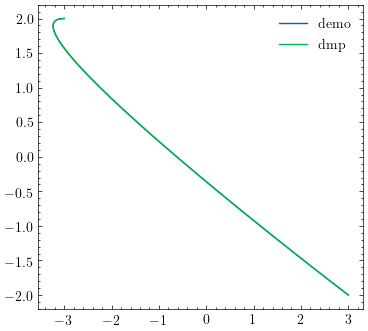
\includegraphics[width=1 \linewidth]{2D_traj.png}
        \caption{2D DMP trajectory}
        \label{fig:2D_traj}
    \end{subfigure}%
    \begin{subfigure}{0.5\textwidth}
        \centering
        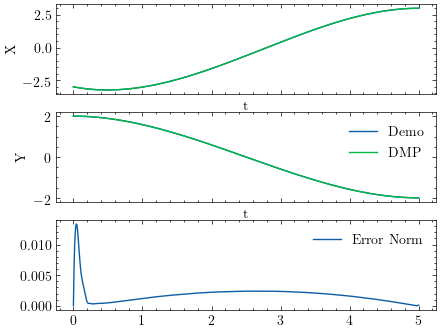
\includegraphics[width=1.2 \linewidth]{2D_traj_error.png}
        \caption{Deviation from the desired trajectory}
        \label{fig:2D_traj_error}
    \end{subfigure}
    \caption{2D DMP trajectory}
    \label{fig:2D_traj}
\end{figure}

\subsection{3D DMP}
Similar to 3D DMP, we can create a 3D DMP in cartesian space by creating a minimum acceleration trajectory for a total time of 5 secs 
between points [-3,-1,1] and [2,3,2] with initial velocity as [0,0,-2].The DMP parameters are: $\alpha_z = 30, N = 100$ with the canonical system parameters as: 
$\alpha_x = 3, \tau = 1$

The resultant DMP trajectory is plotted as shown in Fig. \ref{fig:3D_traj}

\begin{figure}[h]
    \centering
    \begin{subfigure}{0.5\textwidth}
        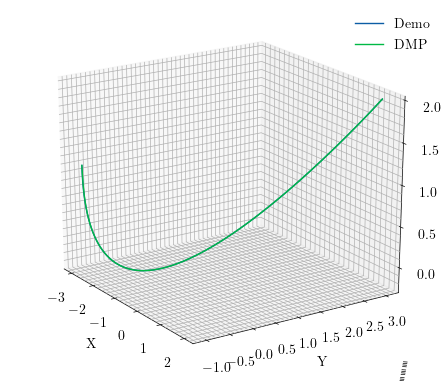
\includegraphics[width=0.9 \linewidth]{3D_traj.png}
        \caption{3D DMP trajectory}
        \label{fig:3D_traj}
    \end{subfigure}%
    \begin{subfigure}{0.5\textwidth}
        \centering
        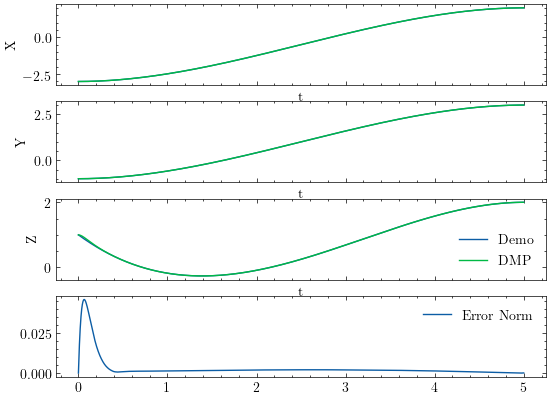
\includegraphics[width=1 \linewidth]{3D_error_traj.png}
        \caption{Deviation from the desired trajectory}
        \label{fig:3D_traj_error}
    \end{subfigure}
    \caption{3D DMP trajectory}
    \label{fig:3D_traj}
\end{figure}

This 3D cartesian DMP can be simulated on a robotic manipulator which follows a certain trajectory.
In this simulation experiment, and all the simulated experiments following, we use Kuka LBR iiwa 
7 axis industrial robot, simulated in PyBullet.
A minimum acceleration trajectory is created between points [0.4,0.4,0.9] and [-0.2,-0.2,1.2] 
 with initial velocity as [0,0.2,-0.1] which has to be travelled in 10 secs. The DMP parameters are:
  $\alpha_z = 20, N = 100$ with the canonical system parameters as: 
  $\alpha_x = 0.5, \tau = 1$

The resultant DMP trajectory simulated is shown in Fig. \ref{fig:3D_only_taj_pybullet}

\begin{figure}[h]
    \centering
    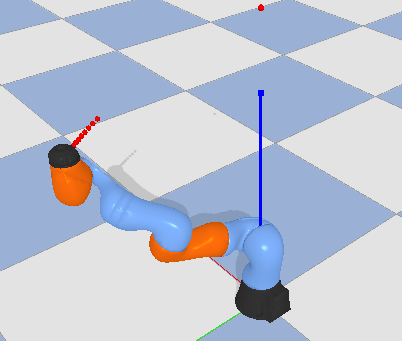
\includegraphics[width= 0.3 \textwidth]{3Dpybullet1.png}\quad
    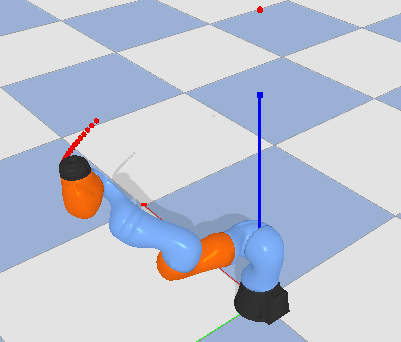
\includegraphics[width= 0.3 \textwidth]{3Dpybullet2.png}\quad
    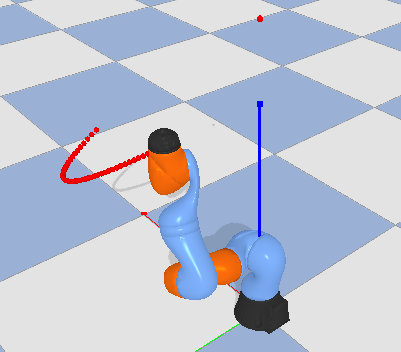
\includegraphics[width= 0.3 \textwidth]{3Dpybullet3.png}

    \medskip

    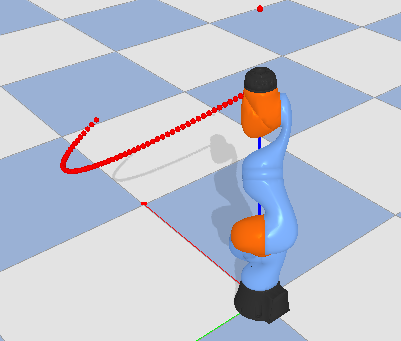
\includegraphics[width= 0.3 \textwidth]{3Dpybullet4.png}\quad
    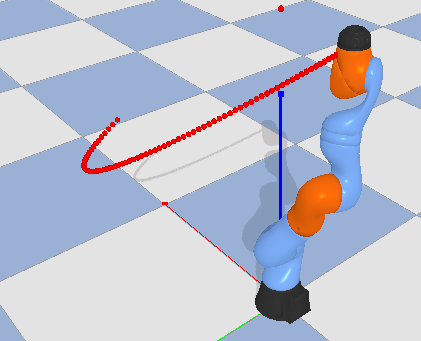
\includegraphics[width= 0.3 \textwidth]{3Dpybullet5.png}

    \caption{3D DMP trajectory simulated on Kuka LBR iiwa 7 axis industrial robot}
    \label{fig:3D_only_taj_pybullet}
\end{figure}

\subsection{Joint Space DMP}
The joint space DMP is a special case where each of the transformation system represents a joint of the robot.
Like previoulsy mentioned the simulation is done on Kuka LBR iiwa. thus the transformation system will be of size 7.
The each joint of the robot follows a sine wave trajectory in time. 

Thus, the desired trajecotry in this case is:
\begin{equation}
    \vect{\Theta(t)} = \vect{\sin(t)} 
\end{equation}
where $\Theta$ is the vector of joint angles and $t \leq T$ where T is the total time of the trajectory.
The parameters of the DMP are: $\alpha_z = 10, N_{bfs} = 1000$ with the canonical system parameters as: 
$\alpha_x = 0.5, \tau = 1$.

The resultant DMP trajectory simulated in DMP is shown in Fig. \ref{fig:joint_traj_pybullet}

\begin{figure}[h]
    \centering
    \begin{subfigure}{0.3\textwidth}
        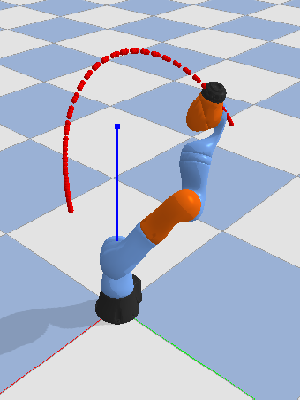
\includegraphics[width=0.9 \linewidth]{jointTraj1.png}
    \end{subfigure}%
    \begin{subfigure}{0.3\textwidth}
        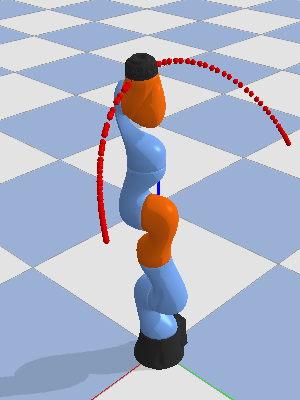
\includegraphics[width=0.9 \linewidth]{jointTraj2.png}
    \end{subfigure}%
    \begin{subfigure}{0.3\textwidth}
        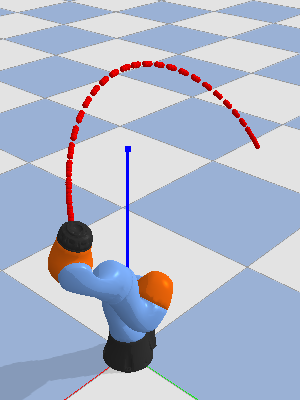
\includegraphics[width=0.9 \linewidth]{jointTraj3.png}
    \end{subfigure}%
    \caption{Joint space DMP trajectory}
    \label{fig:joint_traj_pybullet}

\end{figure}

\section{6DOF }
















